\documentclass[letterpaper]{article}
\usepackage{amssymb}
\usepackage{fullpage}
\usepackage{changepage}
\usepackage{amsmath}
\usepackage{epsfig,float,alltt}
\usepackage{psfrag,xr}
\usepackage[T1]{fontenc}
\usepackage{url}
\usepackage{pdfpages}
\usepackage{epstopdf}
\usepackage[framed,numbered,autolinebreaks,useliterate]{mcode}

%\includepdfset{pagecommand=\thispagestyle{fancy}}
\author{Fan Bu, Feng Zhou, Yi Yang}
\title{ME 552 Lab 01 Report}

\begin{document}
\date{09/17/2016}
\maketitle

\newcommand{\trace}{\mathrm{trace}}
\newcommand{\real}{\mathbb R}  % real numbers  {I\!\!R}
\newcommand{\nat}{\mathbb N}   % Natural numbers {I\!\!N}
\newcommand{\cp}{\mathbb C}    % complex numbers  {I\!\!\!\!C}
\newcommand{\ds}{\displaystyle}
\newcommand{\mf}[2]{\frac{\ds #1}{\ds #2}}
\newcommand{\spanof}[1]{\textrm{span} \{ #1 \}}
\newcommand{\sol}[0]{\textbf{Solution: }}
\newcommand{\pf}[0]{\textbf{Proof:}}
\newcommand{\rme}[0]{\textrm{e}}
\newcommand{\Null}[1]{\textrm{Null}\{#1\}}
\parindent 0pt
%%%%%%%%%%%%%%%%%%%%%%%%%%%%%%%%%%%%%%%%%%%%%%%%%%%%%%%%%%%%%%%%%%%%%%%%%%%%%%%
% Solution for Question 1 begins here - by Yi Yang
%%%%%%%%%%%%%%%%%%%%%%%%%%%%%%%%%%%%%%%%%%%%%%%%%%%%%%%%%%%%%%%%%%%%%%%%%%%%%%%
\section*{Question 1}
\subsection*{(a)}
We design the circuit as shown below:\\
\begin{figure}[h]
\begin{center}
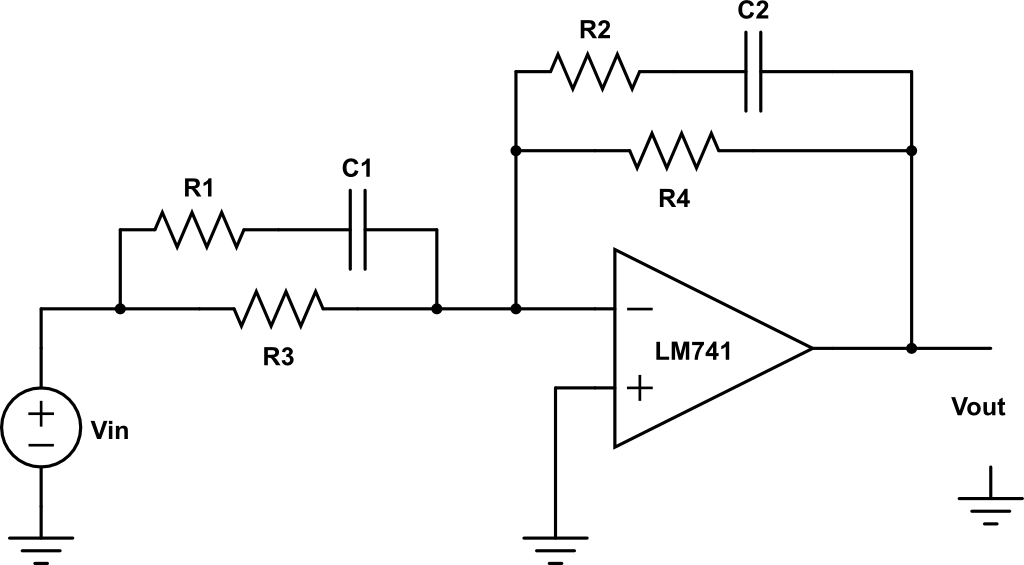
\includegraphics[width=10cm]{q1_circuitDiagram.png}
\end{center}
\caption{A lead-lag compensator circuit diagram for question 1.}
\label{q1_a}
\end{figure}
\subsection*{(b)}
We can let $R_1$, $C_1$, $R_3$ and $R_2$, $C_2$, $R_4$ form two different impedance module separately, and let their impedance equal $Z_1$ and $Z_2$, we can get:
$$Z_1 = \frac{R_3 * (R_1 + (1/sC_1))}{R_3 + (R_1 + (1/sC_1))} = \frac{R_3(sR_1C_1 +1)}{s(R_1C_1 + R_3C_1) + 1}$$
$$Z_2 = \frac{R_4 * (R_2 + (1/sC_2))}{R_4 + (R_2 + (1/sC_2))} = \frac{R_4(sR_2C_2 +1)}{s(R_2C_2 + R_4C_2) + 1}$$
The new circuits can be seen as an inverting amplifier:
$$\frac{V_{out}(s)}{V_{in}(s)} = - \frac{Z_2}{Z_1} = -  \frac{R_4(sR_2C_2 +1)}{(s(R_2C_2 + R_4C_2) + 1)}\frac{(s(R_1C_1 + R_3C_1) + 1)}{R_3(sR_1C_1 +1)} $$
$$=  -  \frac{R_4}{R_3}\frac{(sR_2C_2 +1)}{(s(R_2C_2 + R_4C_2) + 1)}\frac{(s(R_1C_1 + R_3C_1) + 1)}{(sR_1C_1 +1)} $$
If we assume $R_3 = R_4$, we will gain the standard formula of lead-lag compensator.
$$ - \frac{(sR_2C_2 +1)}{(s(R_2C_2 + R_4C_2) + 1)}\frac{(s(R_1C_1 + R_3C_1) + 1)}{(sR_1C_1 +1)}  = \frac{(1+0.1s)(1 + 5s)}{(1+0.01s)(1 + 10s)}$$
As illustrated in Lab1 instruction file, we can use two methods to invert the output polarity, so we could directly get the following equations:
$$R_1C_1 = 0.01$$
$$R_2C_2 = 5$$
$$R_1C_1 + R_3C_1 = 0.01 + R_3C_1 = 0.1$$
$$\implies R_3C_1 = 0.09$$
$$R_2C_2 + R_4C_2 = 5 + R_4C_2 = 10$$
$$\implies R_4C_2 = 5$$
$$\therefore R_4 = R_2 = R_3$$
\subsection*{(c)}
While building this circuit, we made the following assumptions:
\begin{itemize}
\item The op-amps we use are ideal, i.e. the input impedance is infinite and the output impedance is negligible. This implies that the op-amp does not load it's input circuit and loading effects are not seen on the op-amps output terminal.

\item The voltage at the inverting terminal is equal to the voltage at the non-inverting terminal.

\item The open loop op-amp gain is infinite.

\item The op-amp will operate in an ideal manner when the output is not saturated above or below its supply limits.

\item We assumed that the performance of the system is not overly sensitive to variations in resistance and we assumed the values of that the resistors were accurate and that capacitors had negligible internal resistance.
\end{itemize}
\subsection*{(d)}
We can set values to capacitors and resistors arbitrarily. However, the values we can choose for resistors are more flexible than capacitors. Thus, we decide to set the appropriate values to capacitors first and then determine the values of resistors. According to the formulas in section (b), we can choose values as shown below:
\begin{table}[H]
\begin{center}
    \begin{tabular}{|c|c|c|}
        \hline
        \textbf{Component Name} & \textbf{Component Type} & \textbf{Component Specification} \\ \hline
       $ LM 741$                     & \text{Signal Op-amp}         & $ \ V+ = +15V, V- = -15V     $             \\	
       $ C_1$                     & \text{Electrolytic Capacitor}         & $ \ 1 \mu F     $             \\ 
       $ C_2 $                   & \text{Electrolytic Capacitor}         & $ \ 55.55 \mu F     $               \\ 
       $ R_1  $                  & \text{Resistor}         & $ \ 10 K\Omega            $        \\ 
       $ R_2 $                    & \text{Resistor}         & $ \ 90 K\Omega        $            \\        
       $ R_3 $                   & \text{Resistor}         & $\ 90 K\Omega   $                 \\ 
       $ R_4$                     & \text{Resistor}         &$ \ 90 K\Omega$                    \\
        \hline
    \end{tabular}

\caption{Capacitances and Resistances chosen to construct the lead-lag controller}
\label{q1_td}
\end{center}
\end{table}
Having decided on the resistors, capacitors and op-amp that we need, we need further decide the voltage ratings for capacitors and wattage ratings for resistor, the wattage ratings should exceed the power supply of the system to ensure the safety of circuit components.
\subsection*{(e)}
Refer to the "Lab 1 Instructions" document and construct the circuits and collect relevant data.
\end{document}